\setcounter{chapter}{1} 
\chapter{Theoretical Background} \label{ch:theoretical_back}
% Parametrization (atmospheric modeling), a method of approximating complex processes.
\textbf{Rewrite summary when you finished the chapter.}
\textit{This chapter presents the motivation and necessary theoretical background  to understand the need for new methods for estimation cloud cover \textit{(cloud amount)}. Hopefully this will also help shed some light on the understanding of the underlying physical processes. In terms also help reduce the spread in climate sensitivity. Also known as global mean temperature increase in future climates. The data used in this project is a combination of satellite retrievals and reanalysis data.}
\\ \\
Starting with giving a introduction to clouds in the current and future climate. Continuing with information about the dataset, structure, implementations and practical implications.
\section{Clouds role in the climate system} \label{sec:cloud_in_climate_system}
% Clouds, climate and machine learning
Clouds play an important role in the climate system. Both affecting the radiative budget and the hydrological cycle. Understanding how clouds form in the complex system of the atmosphere involves both knowledge about the large scale influence by the circulation and the small scale influenced by aerosols. Clouds are composed of liquid droplets, ice crystal or both. To this day the micro-physics of all phases are not fully understood. Here mixed phase clouds, consisting of both liquid and ice, shows to be the most difficult. 
%Climate models are the most useful tool for studying the past, present and future climate. Clouds and aerosols are acknowledged as the factors contributing with the largest uncertainty to the \acrfull{ecs}. Also known as global mean temperature increase as a consequence of doubling of the pre-industrial levels of $CO_2$ (280 \acrshort{ppm}). \textbf{kilde AR4 which ch?} \textit{It remains unclear to which level of sophistication is adequate to model their effect om climate.} (\cite{IPCC_CH7_clouds}).

%\textbf{Make sure you include everything that's related to parametrised processes.}
It is understood that cloud formation requires suitable aerosols and sufficient supersaturation. \textit{Aerosols} include both gases and solid particles suspended in air. They interact with the clouds by serving as particles which vapour and ice can condensate or deposit upon. The different phases require different properties and the nuclei are called \acrshort{ccn} for liquid droplets and \acrshort{inp} for ice crystals. Saturation is usually achieve by a temperature decrease in rising air masses. %Thus the stability of the atmosphere  plays a key role for convective motions.
%\textbf{Legg inn bilde a skyer en i is fase og en i liquids. Skriv noe som "the sharp outoline suggest that the cloud is consisting of liquid droplets, even at temperagtures below 0."}
%The negative temperature decreases by height is often referred to as the lapse rate, $\Gamma_{s, d}$. 
 
Growth processes are phase dependant. Liquid droplet grows by diffusion and later by collision and coalescence. At temperatures -38 $^oC$ (\cite{lohmann2016}) they will spontaneously freeze and could play the role as INP. 
%When both phases are present in a cloud, the saturation vapour pressure over ice is higher than over liquid. This may cause the droplets to evaporate and deposit on to the ice crystals. 
This mechanism exist because the saturation vapour pressure is lower with respect to ice than water. It is most efficient at 12$^oC$ when the difference is largest. This is called the Wegeron-Bergeron-Findeisen process. Clouds consisting purely of ice crystals first grow by deposition of vapour then by aggregation (\cite{Fowler1996LiquidAssumptions}). 

% Lots of different processes occurring simultaneously on different scales 
The complex nature of clouds originates from lots of different processes occurring simultaneously on different scales. Incorporating all these interactions into a model framework has proven to be difficult (\cite{IPCC_CH9_climate_models} +++ ). \textbf{Finn multiple sources} 

\section{Clouds in the current climate} \label{sec:intro_cloud_current_climate}
Based on satellite and ground based measurements \cite{Wild2019TheModels} have quantified the contribution of elements in the radiative budget. Cloud radiative effect (\acrshort{cre}) in earth annual mean energy budget between a cloudy and a cloud-free atmosphere. This is shown in equations \eqref{eq:cre_sw} and \eqref{eq:cre_lw}. \textbf{drop equations..?}
\cite{Wild2019TheModels} concludes with a reduction in shortwave radiation of $-47Wm^{-2}$ by clouds. In other words clouds reflect approximately 50\% of the incoming solar radiation. Longwave component is $28Wm^{-2}$. This give a net \acrshort{cre} of $-19Wm^{-2}$. Proving that the net effects of clouds on the radiative budget is negative.The altitude along with the composition determines the radiative properties of the cloud. 

\begin{figure}[h]
    \centering
    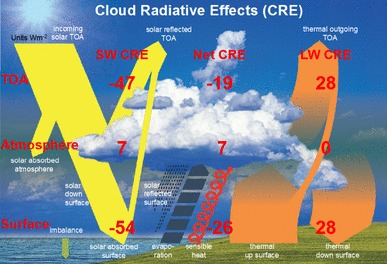
\includegraphics[scale = 7]{Chapter1_Intro/images/CRE_wild2019.jpg}
    \caption{Cloud radiative effect, CRE is the difference between the radiative components of the Clear sky radiative and the all sky. Modified version of as Figure 15 in \cite{Wild2019TheModels}. \textbf{pappa syns denne var grusomt vanskelig.}}
    \label{fig:cre}
\end{figure}

\begin{equation} \label{eq:cre_sw}
    CRE_{sw} = SW\uparrow_{clear-sky} - SW\uparrow_{all-sky}
\end{equation}

\begin{equation} \label{eq:cre_lw}
    CRE_{lw} = LW\uparrow_{clear-sky} - LW\uparrow_{all-sky}
\end{equation}

\begin{equation} \label{eq:stefan-boltzmann}
    F = \sigma \epsilon T ^4
\end{equation}

The physical properties causing the interaction with radiation is described below. Dense low level clouds reflect solar radiation. This is called the albedo effect. \textit{Albedo} being the ratio between reflected to incoming radiation. The higher number concentrations of droplets in a cloud the higher the total surface area of droplets. The more radiation gets reflected back into space. Clouds absorb longwave radiation and re-emits it. The absorbed radiation originates from the surface and is given by Stefan-Boltzmann forth-power law, see equation (\ref{eq:stefan-boltzmann}). The emissivity, $\epsilon$ depends on the (composition, compactness and surface roughness) of the medium. Water, snow and ice have different spectral emissivity (\cite{Huang2018ImprovedClimate}). Different parts of the globe are covered by different surfaces and \citeauthor{Huang2016AnSimulations} proved that assuming a constant surface emissivity effects the \acrshort{toa} polar energy budget. The greenhouse effect increases with the cloud altitude. Since high clouds have low temperatures and since the re-emitted radiation at a lower intensity than they absorbed. Researchers are still working on determine the emissivity of the different phases. Despite the uncertainties related to emissivity of the medium, the re-emitted radiation is of a lower intensity than what it absorb.

\section{Clouds in future climates} \label{sec:intro_cloud_future_climates}
\begin{figure}[h]
    \centering
    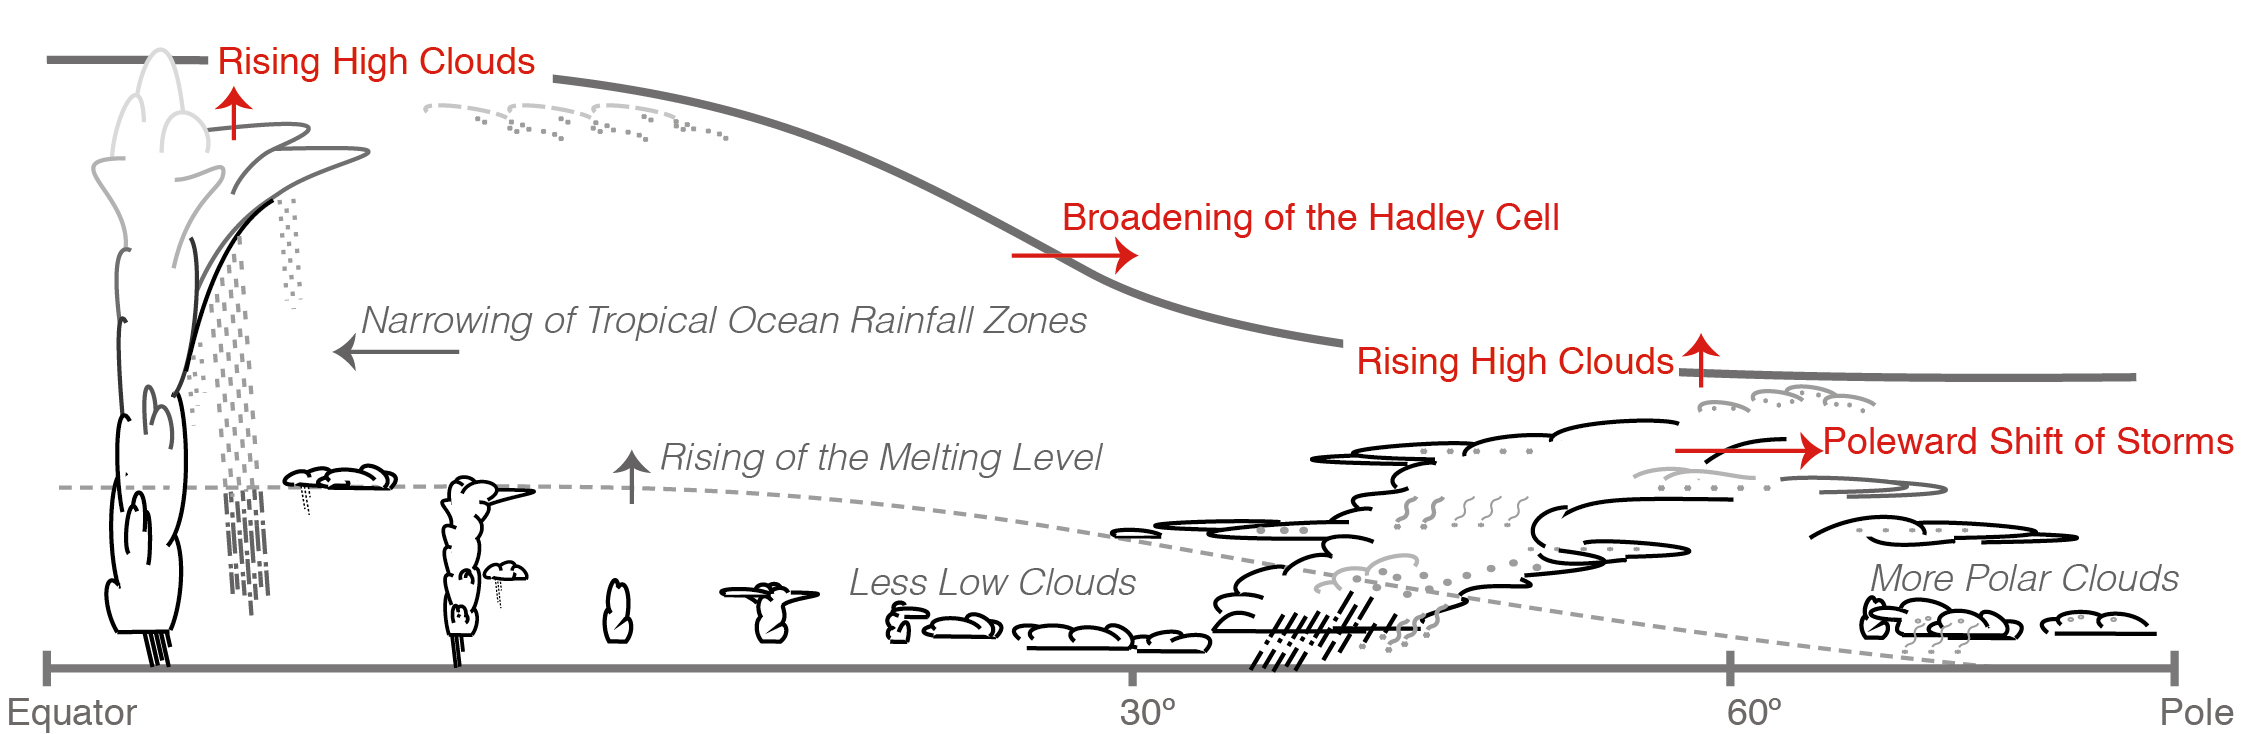
\includegraphics[scale = 0.8]{Chapter1_Intro/images/Fig7-11_ipcc.jpg}
    \caption{Cloud climatology in future climate. Developed based feedback's in climate models, the different adjustments have different uncertainty (\cite{IPCC_CH7_clouds}).}
    \label{fig:cloud_scheme}
\end{figure}

Excess of radiation gets trapped in the earth system, forcing the surface temperature to increase in order to close the radiative budget. The imbalance at the \acrfull{toa} is estimated by \cite{Wild2019TheModels} to be $0.6W m^{-2}$. 
% Wild et. al. 2019  \textbf{siter} finds an imbalance of This heat gets trapped in the earth system, forcing the surface temperature to increase in order to close the radiative budget. 
%The imbalance in the radiative budget at \acrfull{toa} is the radiative forcing. 
Climate drivers include both natural and anthropogenic forcings. \textit{Forcings} can be everything from natural variability in the solar energy output, volcanic eruptions and greenhouse gas emissions. The climate science community works toward a common goal to determine the climate sensitivity as a function of forcing. Different socio-economic pathways result different \acrshort{ecs}. The temperature increase induces climate changes. The \acrfull{ipcc} (\cite{IPCC_CH7_clouds}) suggest the following shift in cloud schemes (see figure \ref{fig:cloud_scheme}). Figure \ref{fig:cloud_scheme} shows a summary of the most likely cloud feedback's. First, a broadening of the Hadley cell causes a poleward shift of storms. This dries up the subtropics and moistens the higher latitudes. The clouds move further into the polar night, decreasing the albedo effect. The greenhouse effect of clouds still persist without sunlight leading to a net heating in the Arctic. Second, rising higher clouds causing a stronger greenhouse effect. Third, less low level clouds. This is assumed to be partly offset by a increase in the melting layer, leading to more opaque clouds. Rising of the meltlayer cause ice crystals to melt resulting in more opaque clouds. These opaque clouds have a higher albedo and reflect more sunlight. 
%\subsection{Cloud feedbacks from convection and fronts} %Cloud, circulation and climate sensitivity article.

\section{Parametrisation of clouds} \label{sec:param_clouds}
Parametrisation are a tool used in climate models to include the effect of subgrid-scale processes. This is done for several processes \textbf{give examples - michrophysics Lohmann}. This thesis is only concerned with parametrisation of cloud cover. The simplest form of cloud scheme is binary. Either the entire pixel is covered by clouds or there is no clouds. This can be implemented as follows,
\begin{equation} \label{eq:binary_param_clouds}
    CLA\left(RH\right) = 
     \begin{cases}
       \text{0,} &\quad\text{if RH}\le100\\
       \text{1,} &\quad\text{else}
     \end{cases}
\end{equation}
Sub-grid scale variability in humidity is necessary to archive fractional cloud cover. This can be combined with a sub-grid scale of temperature. Over the years researchers have tried to draw the distributions of these variables from observations and implement them into models. Virtually all probability density functions, PDF's have been used to model either cloud cover or its dependant variables humidity, temperature and so on. They have not been successful in finding a adequate representation of cloud cover using this approach. \textbf{(siter Tomkins summary)}. Cloud cover is usually a combination of several parametrisations. Its common to have separate schemes for ice-, liquid clouds and convective clouds. \textbf{Read more Tomkins}
\\ \\ 
%What is necessary to understand why clouds are Parameterisations. Cite that all climate models are wrong but some are useful.
\subsection{Parametrisations of clouds - Climate models} \label{sec:params_climate_models}
\textit{Trude: Most climate models have a fractional cloud cover, which is driven by saturation threshold. In global climate models all michcrophysics (bilde lohman), convection are parametrised in dependant structures. Climate models output monthly mean/or et tidspunkt hver måned.}
\textbf{Include details on parameterisations in climate models}
\\ \\ 
One method to deal with this is cloud parameterisation are cloud resolving models. This runs a LES-model. You still need to parametrise the michrophysical scheme, but the model might be able to resolve the convection. \textbf{Read paper.}
% Climate models are an important tool for studying the effects of emissions/forcing on future climates. The \acrfull{ipcc} provide assessments report every ~10th year or so, providing a state of the art status update on the current knowledge of climate change. Since the previous assessment report there has been three special report A, B and C. \textbf{Les special report.} The previous report published was Assesment report 5, AR5 in 2013 and the next report is scheduled to be published in 2021. 
%The ensamble of climate models included in AR5 is \acrfull{cmip5}. \acrshort{cmip6} are now being evaluated, thus there is less published literature. Even though its a bit old, we will mostly focus on the results in AR5. \textbf{Plus the findings in the special reports.}
\\ \\
In resent years a lot of effort have been invested in improving the parametrisations of sub-grid scale processes. Among these clouds contribute with the largest uncertainty, approximately three times as large as other process i.e. relative humidity-lapse rate feedback (these processes should not be viewed in isolation). The contributions of the clouds to the short wave component in the radiative budget is the main contributor to the uncertainty. Short wave cloud feedback. \textit{To this day neither observations of \acrfull{gcm} provide clear evidence or contradict the low level clouds feedback}. There is no accepted basis to refuse a \acrshort{gcm} \textit{a priori} \textbf{this increases the multi-model mean spread in climate sensitivity}. Missing representations of clouds micro-physical processes related to opacity or cirrus (high altitude, composed of ice) clouds. \textbf{cite AR5}
\\ \\
The computational cost of generating these large ensembles are limiting factor. Simplified models in terms of resolution and/ or complexity is common/often necessary. 
\\ \\ 
Using idealised experiments they give model spread in \acrfull{ecs}. This describes the \textit{equilibrium change in global and annual mean surface temperature after doubling the $CO_2$ conditions from pre-industrial times.} For \acrshort{cmip5} the \acrshort{ecs} is $2.1^oC$ to $4.7^oC$. The is very high confidence that clouds are the primary factor attributing to the wide range. This is not a very big improvement from Hansen et. al. 1984 first estimate of climate sensitivity which was the range $2.0^oC$ to $5.0^oC$. \textbf{explain idealised experiments.} Hansen et. al. ran their experiments using a coarse resolution of $8^o \times 10^o$ grid box (lat $\times$ lon) and a doubling of the $CO_2$ concentrations from 315ppm to 630ppm. 

\subsection{ERA5 - make sure this should be included before you write it} \label{sec:param_ERA5}
ERA5 is produced used IFS cycle 4lr2. This has a new cloud scheme or hydrological cycle. \textbf{Artikkelen forteller om oppdateringer fra sist era-interim produksjon ikke alt som finnes. Bedre å skrive denne etter du har skrevet i datasettet hvor }. Husk Tomkins jobber for ECMWF.

\section{Dataset and Methods}
\subsection{ERA5} \label{sec:era5}
ERA5 is the latest in the series of reanalysis produced by \acrfull{ecmwf}. Re-analysis is as close to observations as one can get coherent in space and time. It is produced using a forecast model to assimilate observations. Data assimilation take observations and input and tries to make a accurate estimate of the state of the system. This includes observations from ground based, ships, bouyes, airplanes and satellites. The analysis is produced in the operational system, making it available within five days of real time. ERA5 is based on the Integrated Forecasting System, IFS cycle 4lr2. The data is available in $0.25^o$ degree and hourly resolution. Its an important product for the continuous climate monitoring of the earth system. It can be wort noting that the all sky radiance's from \acrfull{msg} in the period 2003-2012 is included in the assimilation. This is the same satellite that provides the cloud mask. 
\\ \\ 
Reanalyses data is often mistakenly referred to as observations. This was the theme of a essay in \acrfull{bams}, 2015. Based on the following three points they conclude that observations and re-analysis are not to different. First, both involve inference (theory based calculations). Re-analysis relies on forecast and observations does not. Second, it is not a significant difference as long as the forecast is sufficiently accurate. Third, its important to be aware of that the uncertainty of the reanalysis is less well known than for observations. This makes it harder to judge appropriate use of the reanalysis. 
\textbf{One sentence explaining that we have judged the appropriate use and have come to the conclusion that using the assimilated variables and not parameterised are appropriate for this application.}
\\ \\
\subsection{Remote sensing of cloud properties}
Satellites are instruments capable of providing continuous global measurements. Two types of sensors, passive and active imagers. The passive imaging sensor detects natural occurring levels of radiation. Opposed to active sensor, which detect the radiation returned from a emitted artificially fixed pulse of radiation.

\begin{figure*}
        \centering
        \begin{subfigure}[b]{0.475\textwidth}
            \centering
            \includegraphics[width=\textwidth]{Chapter2_Theory/images/sat_channels/meteosat-msg_wv062_overlay-ne_10m_coastline_overlay-ne_10m_admin_0_boundary_lines_land.png}
            \caption[Channel WV 6.2]%
            {{\small Channel WV 6.2}}    
            \label{fig:WV_6.2}
        \end{subfigure}
        \hfill
        \begin{subfigure}[b]{0.475\textwidth}  
            \centering 
            \includegraphics[width=\textwidth]{Chapter2_Theory/images/sat_channels/meteosat-msg_vis006_overlay-ne_10m_coastline_overlay-ne_10m_admin_0_boundary_lines_land.png}
            \caption[]%
            {{\small VIS 0.6}}    
            \label{fig:VIS_0.6}
        \end{subfigure}
        \vskip\baselineskip
        \begin{subfigure}[b]{0.475\textwidth}   
            \centering 
            \includegraphics[width=\textwidth]{Chapter2_Theory/images/sat_channels/meteosat-msg_ir108_overlay-ne_10m_coastline_overlay-ne_10m_admin_0_boundary_lines_land.png}
            \caption[something]%
            {{\small IR 10.8}}    
            \label{fig:IR_10.8}
        \end{subfigure}
        \quad
        \begin{subfigure}[b]{0.475\textwidth}   
            \centering 
            \includegraphics[width=\textwidth]{Chapter2_Theory/images/sat_channels/meteosat-msg_ir039_overlay-ne_10m_coastline_overlay-ne_10m_admin_0_boundary_lines_land.png}
            \caption[]%
            {{\small IR 3.9}}    
            \label{fig:IR_3.9}
        \end{subfigure}
        \caption[ The average and standard deviation of critical parameters ]
        {\small Spectral bands from SEVIRI. February 15th 2020 at noon. It shows the lowpressure system \textit{Elsa} persisting over iceland. Having a record breaking low of 914hPa. \textbf{NRK artikkel} 
        % info på bildene \textbf{Rectified (level 1.5) Meteosat SEVIRI image data. The data is transmitted as High Rate transmissions in 12 spectral channels. Level 1.5 image data corresponds to the geolocated and radiometrically pre-processed image data, ready for further processing, e.g. the extraction of meteorological products. Any spacecraft specific effects have been removed, and in particular, linearisation and equalisation of the image radiometry has been performed for all SEVIRI channels. The on-board blackbody data has been processed. Both radiometric and geometric quality control information is included. Images are made available with different timeliness according to their latency: quarter-hourly images if latency is more than 3 hours and hourly images if latency is less than 3 hours (for a total of 87 images per day). To enhance the perception for areas which are on the night side of the Earth a different mapping with increased contrast is applied for IR3.9 product. The greyscale mapping is based on the EBBT which allows to map the ranges 200 K to 300 K for the night and 250 K to 330 K for the day.}
        % Lastet ned 16.02.2020.
        \href{https://eumetview.eumetsat.int/mapviewer/?product=EO:EUM:DAT:0025}{https://eumetview.eumetsat.int/mapviewer/?product=EO:EUM:DAT:0025}
        \href{https://www.nrk.no/nordland/nytt-lavtrykk-kan-skape-trobbel-for-wideroe-og-flytrafikken-i-nord-norge-1.14902193}{https://www.nrk.no/nordland/nytt-lavtrykk-kan-skape-trobbel-for-wideroe-og-flytrafikken-i-nord-norge-1.14902193}} 
        \label{fig:SEVIRI_channels}
    \end{figure*}
Karlsson et. al. 2015 list the five key properties for remote sensing of clouds using passive imagery. To have a reference figure \ref{fig:SEVIRI_channels} shows examples on how different properties are seen by the satellite. This includes the four spectral bands, WV 6.2, VIS 0.6, IR 3.9 and IR 10.8. In general anything that appears bright have a higher reflectance at the \acrfull{toa} than the surface. Lower radiences are displayed in darker colours and brighter is white. Clouds appear bright in VIS and NIR channels, see \ref{fig:VIS_0.6}. Clouds consisting of liquid droplets reflect strongly in SWIR and MWIR. This is shown in figure \ref{fig:IR_3.9}. The earth surface, including snow and ice, appear dark. This allows for detection of low level clouds at night. Exploiting the fact that clouds are not perfectly emitting black bodies. Cloud are typically colder than the earth surface. Cirrus cloud are optically thin, but can be detected using split window channels (IR10.8 and IR12.0) differences. See figure \ref{fig:IR_10.8}. Figure \ref{fig:WV_6.2} shows detected water vapour. In general broken clouds give rise to scattered pattern or texture in images otherwise homogeneous, ice-free ocean for instance. To summaries the success of a screening is dependant on the illumination, the state of the surface and atmosphere. \textbf{kalsson et al} The number of spectral bands and footprint size (pixel resolution) determine the practical application a particular retrieval can be used for. Differences in swath width determine the frequency at a given position. Viewing angle affect the optical properties of the medium (but also its apparent position). \textit{Parallax} describes the apparent shift in position of a object, when you move the observer along a axis. This is a issue in remote sensing. Positions of satellites are moved and high viewing angles may cause similar issues. Since the position of objects is relevant to the viewing angle. A high viewing angle may introduce problems with parallax of high clouds. This factor is negligible when detecting low clouds (Joro et al). Moving the observer (satellite) changes the apparent position of the measurement. This becomes evident when comparing simultaneous measurements for the operation and the standby METeosat satellites.
\\ \\
Differences in sensitivity and retrieval algorithms contribute to a large spread in global mean cloud amount among different cloud products. In their assessment of global cloud datasets Studbenau et. al. 2013 compared the global mean cloud cover of six datasets (ISCCP, PATMOS-x, MODIS-ST, MODIS-CE, AIR-LMD and TOVS Path-B). In this process they eliminating MISR and ATSR-GRAPE because of different observation times \textbf{(ref the table in the article)} and two outlier datasets, HIRS-NOAA and POLDER. Their results show that the difference among the six datasets, the difference is of order 0.08. On the contrary, local differences could be up to 0.4. Its worth noting that the satellite data using in this thesis is not included in Schubanaus study, but its illustrates nicely the large differences among other datasets. 
\\ \\ 
Spatiotemporal consistency and resolution was given high priority when choosing a dataset. %Main goal is to gain insight to cloud dynamics (..?) using a physical based parametrisation. 
Cloud cover is a two dimensional variable. This results in a larger pool av satellites to chose from. The satellite product chosen for this thesis is the \acrfull{msg}. This is geostationary, has a exceptional temporal resolution. Knowing that the average lifetime of a cloud is 60min or less, it seems like a reasonable choice. \textbf{kilde Lohmann s.19}
%Cloud-Aerosol Lidar and Infrared Pathfinder Satellite Observations, CALISO is much used in other research because it gives a vertically resolved cloud (3D observations). This additional spatial information is provided on the expense of frequency and uncertainty. \textit{Reason why calipso is ruled out as a candidate. large uncertainty Stubenau} MODIS has low spatial resolution but high temporal resolution, one to two days. National Oceanic and Atmospheric Administration, NOAA \textbf{ something}. Most polar orbiting satellites have a resolution at best daily. \textbf{kilde (shubenau)} \textbf{Does the other one give ferdig produkter av skyfraksjoner og eller er mye lettere og regridde??} The number of channels (higher for other than METEOSAT). The more channels you have the more accurate cloud detection algorihms you can use. Most of the uncertainty in satellite retrivals are attributed to the presence of clouds.  
\\ \\
\subsection{METeosat Second Generation, MSG} \label{sec:meteosat}
Prior to the launch of the METeosat researchers discussed the temporal frequency suitable for the observing weather. The METeosat first generation had a temporal resolution of 30min \textbf{kilde}. For the second generation, 15min intervals was chosen to best cope with the short lifetime and rapid deformation of clouds. It was also suggested that a temporal frequency of 1 to 10min is necessary tracking cumulus type clouds. \textbf{kilde stubenau - må være en annen kilde}. This agrees with the table 1.3 in Lohmann et. al. stating the lifetimes of different type clouds. \textbf{kilde Lohmann s. 19} There is a \textit{ring} of geostationary satellites located at equator providing a global covering (not included polar regions). The altitude of satellite determine the forward velocity and is chosen for the geostationary orbit. To achieve this orbit it needs to maintain a height of $\sim 36 000km $. The first Meteosat Second Generation (MSG-1) was lauched 28 August 2002. It became operational 29 January 2004 and got renamed Meteosat-8. The \acrshort{msg} system provides a two satellite system, one operational and one standby. The operational satellite at a nadir point of $0^o$ latitude. Samples a full disk in cycles of 15min. A full disk is $3712\times 3712$ pixels.
%\textbf{Thoughts:}
%\begin{enumerate}
%    \item Would it be possible to see further north if the altitude where higher? (Wouldn't be geostationary anymore but would you.)
%    \item Må den alltid være på latitude = 0 for å være geostationary? 
%\end{enumerate}
\\ \\ 
%METeosat is the only geostationary satellite covering the Europe, Africa and India?. Geostationary \textit{ring} of GEO-satellites. 
The \acrfull{msg} was established as a corporation between \acrfull{esa} and \acrfull{eumetsat}. \acrshort{esa} was in charge of developing the prototype of MSG-1. \acrshort{eumetsat} is responsible for maintaining the user requirements, launch procedures, developing ground segments, ensuring over all system consistency and day to day operations.  \acrshort{msg} primary function is to provide a continuous observations of the earths full disk. Near-constant sampling frequency and a geostationary orbit allows for observing weather phenomena occurring on short scales. Since the satellite always is located at $0^o$ the spatial resolution is not constant spatial resolution, unlike the polar orbiting satellites. The resolution becomes coarser with increasing off-nadir viewing angle. \textbf{kilde stubenau} There are efforts invested in extending the MSG dataset with the MFG, in order to make use of the timeseries all the way back to 1980. \textbf{kilde, launched 1977} This is requires new cloud detection algorithms since they only have three common channels and two of them are useful for detecting clouds. \textbf{kilde Stöckli} This could potentially be useful in the future. 
\\ \\ 
On board the \acrshort{msg} is the \acrfull{seviri} imaging radiometer. Its has  12 spectral channels. The scan is done south to north, east to west. The wavelength of the discrete channels are chosen based on heritage from other sensors. One broadband visible channel, three solar channels (0.6, 0.8 and 1.6 $\mu m$) and 8 thermal infrared channels (3.9, 6.2, 7.3, 8.7, 9.7, 10.8, 12.0 and 13.4 $\mu m$). (Taravat, 2015)  This is of great advantage since much of the community already know how to use the \acrshort{seviri} radiance observations. The channels have been chosen based on their ability to detect clouds, water vapour and ozone. More information about what the different channels detect is available in this paper \textit{An introduction to METeosat second generation (MSG)} published in BAMS 2002 \textbf{kilde Schmetz}. % \ref{tab:dataset_summary}.  \\ \\
\begin{figure}[h]
    \centering
    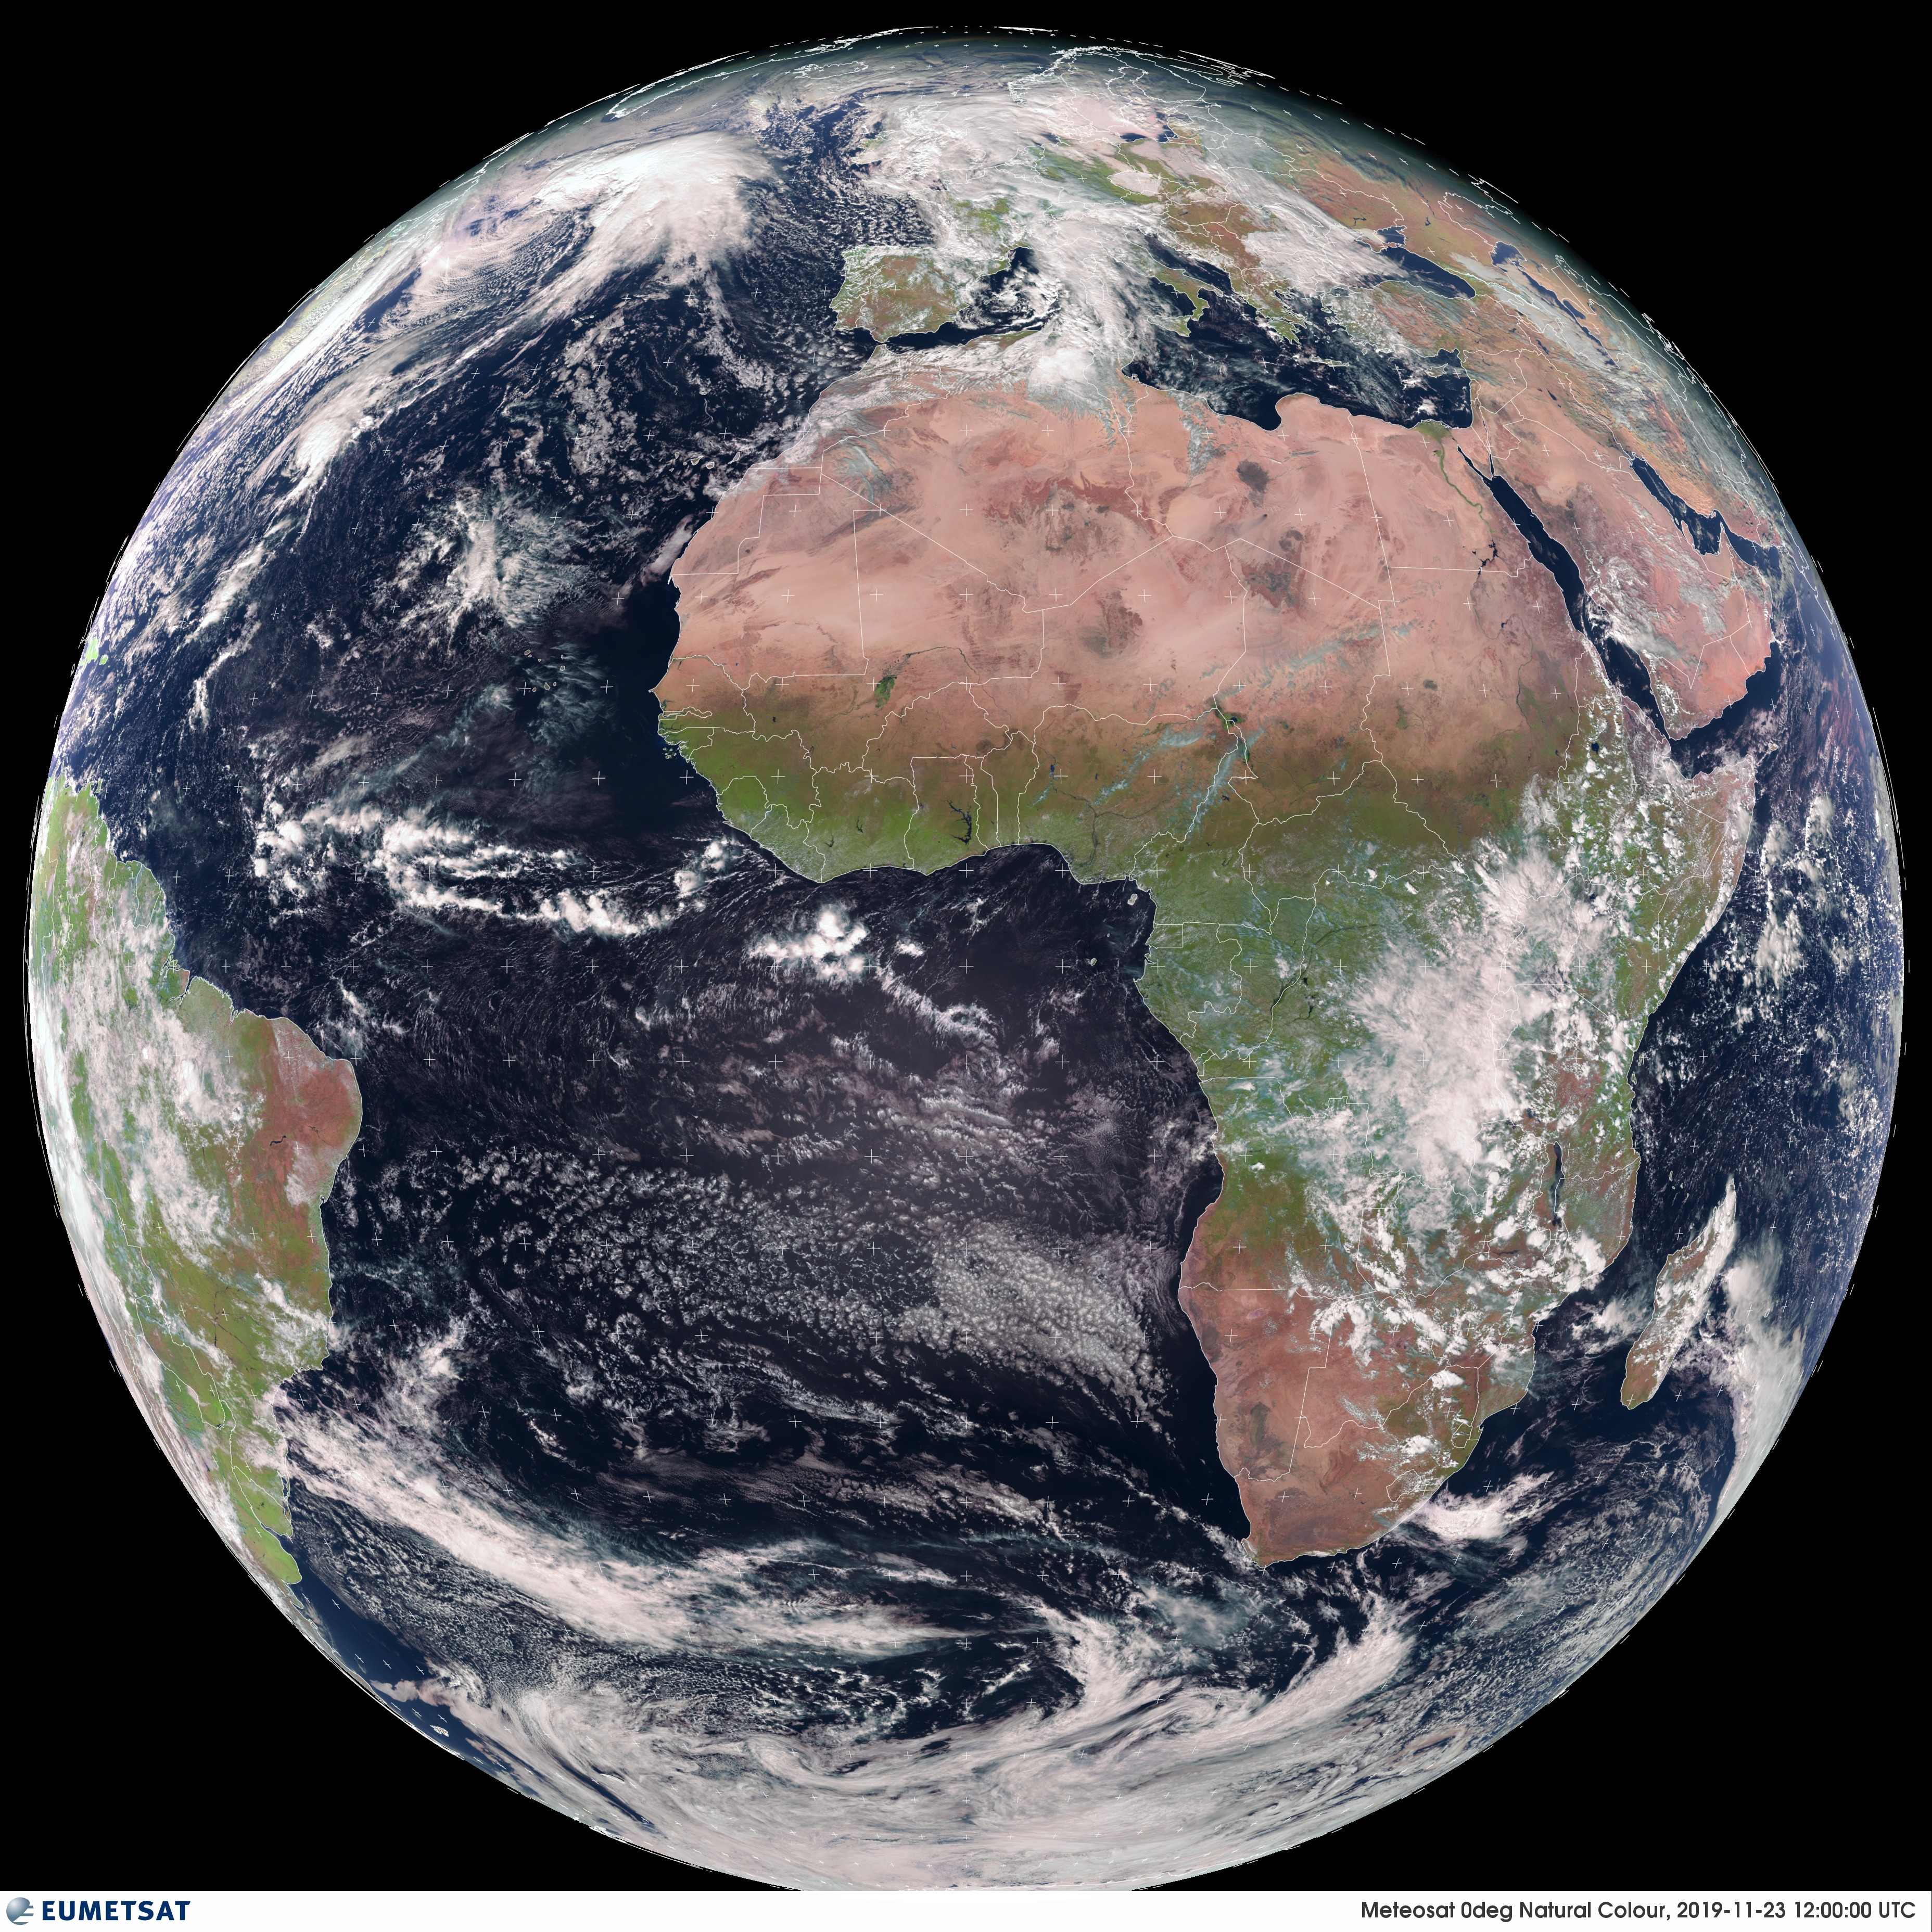
\includegraphics[scale=0.11]{Chapter2_Theory/images/MET10_RGBNatColourEnhncd_FullResolution_20191123120000.jpg}    
    \caption{\textit{Coverage with \acrshort{seviri} on MSG.}The view of the earth from \acrshort{msg}. The picture is dated noon on the 11 November 2019. \textbf{Cite EUMETSAT}. By studying the patterns it becomes evident that clouds are influenced by the circulations. The image is "Natural colors enhanced"}
    \label{fig:sat_view}
\end{figure}
%You may calculate the difference of the measurements, e.g. for channels VIS0.6, IR3.9 and IR10.8 between the two satellites. This will give an estimate how large the measurements differ and as a consequence the products (e.g. cloud mask) will be different.\textbf{also personal corespondance.}
The last couple of years researchers have been investigating the potential of using deep learning algorithms in order to include the spatial structures. This is lost in today's pixelwise detection. \textbf{List many sources}.
\\ \\
\subsection{EUMETSAT Cloud Mask} \label{sec:EUMETSAT_cloud_mask}
The \acrshort{eumetsat} cloud mask, CLM consist of four classes, see table \ref{tab:classes_clm}.

\begin{table}[]
    \centering
    \begin{tabular}{c|c}
        Class & Description \\ \hline
        0 & Clear sky over ocean \\
        1 & Clear sky over land \\
        2 & Cloudy \\
        3 & No data/ outer space        
    \end{tabular}
    \caption{Description of classes in EUMETSAT Cloud Mask product.}
    \label{tab:classes_clm}
\end{table}

\begin{table}[]
    \centering
    \begin{tabular}{c|c}
        Spectral band & Central wavelength $\left( \mu m  \right)$ \\ \hline
        VIS 0.6 & 0.635 \\
        VIS 0.8 & 0.81 \\
        NIR 1.6 & 1.64 \\
        IR 3.9 & 3.92 \\
        WV 6.2 & 6.25 \\
        WV 7.3 & 7.35 \\ 
        IR 8.7 & 8.7 \\
        IR 9.7 & 9.66 \\
        IR 10.8 & 10.8 \\
        IR 12.0 & 12 \\
        IR 13.4 & 13.4 \\
        HRV & 0.75
    \end{tabular}
    \caption{List of MSG spectral bands and their central wavelength. \textbf{Expand this with a column of what they are useful to detect. Move table to MSG section. } All of these channels are useful when detection clouds except on? Add subplots of images in the different channels. See Schmetz et. al. 2002  Not refered to anywhere yet.}
    \label{tab:msg_spectral_bands}
\end{table}
These classes are derived from almost all channels except HRV and isolated pixels are reclassified \textbf{cite article 10 in Tavarat, 2015}. The cloud mask is distributed in GRIdded Binary or General Regularly-distributed Information in Binary form (GRIB) (no coordinates) and network Common Data Form (NetCDF) (coordinates). The data is available on Earth Observation Portal on EUMETSATS web pages. 
\\ \\ 
The viewing angle attributes to small differences in detected cloud mask. Explained by parallax. This becomes evident when the standby and operational satellite scan simultaneously. By default the standby satellite is adjusted to fit the position of the operational. By taking the difference some small patterns becomes visible. This is not accounted/adjusted for when using the data. Sometimes both satellites gather data at the same time. Then the standby-satellite grid is rectified to a a grid of the operational one \textbf{(Personal correspondence EUMETSAT staff).} 

\subsection{European Cloud Cover} \label{sec:ecc}
\acrfull{ecc} comprises of five variables collected from two sources; ERA5 and EUMETSAT. Preserving the resolution available from ERA5. Remapping the cloud mask to cloud fractions. The final product consist of the variables temperature, pressure, cloud amount, specific and relative humidity. Hourly data on a $0.25^o$ uniform grid  resolution in the period \textbf{put in first date} to \textbf{last date}. The original data is described in table \ref{tab:dataset_summary}. Total cloud cover is produced from area weighting cloud masks. The others are on their original format as provided by \acrfull{ecmwf}. A summary of the original sources of the dataset is given in table \ref{tab:dataset_summary}.
\\ \\
The regridding functionality was implemented in Python and is publicly available though the project GitHub. Running the code for all year takes a while on a regular computer. Each time step is stored in individual grib-files. One netCDF-file is stored for its coordinate-information. Its done like this because of storage limitations. One netCDF-file take up roughly 1GB of memory. For more details concerning remapping see section \ref{sec:remapping}. 
\\ \\
% Present Domain
For this project the geographical domain has been restricted latitude $\in[30,50]$ and longitude $\in [-15, 25]$. This becomes $80\times160$ pixels for each time step. As always when working with observations, data is missing. This is either individual pixels of entire disks. Since the individual pixels are remapped to fractions by using the area weighted mean, NaN's are not a issue. When the entire disks are missing, the closest time step available within the previous and trailing 45 minutes are chosen. Other gaps are documented in \textbf{X}. The finished product is named \acrfull{ecc}.
\begin{figure}[h]
    \centering
    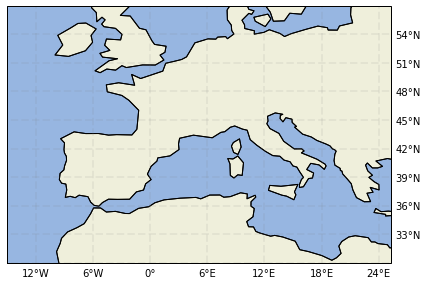
\includegraphics[scale = 0.7]{Chapter2_Theory/images/Domain.png}
    \caption{Map showing the domain. The region cover southern Europe and northern Africa. The coordinate system is Plate Caree, which is the same as ECC. The image have been generated using the python package cartopy ref? \textbf{new figure with correct range and some vegetation or topography on  } \textbf{generate new plot with the updated boundaries}}
    \label{fig:map}
\end{figure}
The mapping from the curve-linear grid of the geostationary satellite to the uniform grid of era5 is quite cumbersome, for more details see section \ref{sec:regridding}. The cloud amount of a pixel is the sum of the area weighted cloud mask contributing to a cell.
\begin{table}[]
    \centering
    \resizebox{\textwidth}{!}{%
\begin{tabular}{c|c|c|c|c|}
\cline{2-5}
\multirow{4}{*}{}                                 & \multicolumn{2}{c|}{\textbf{ERA5}}                                                                                                   & \multicolumn{2}{c|}{\textbf{MSG2}}                                                                                                                \\ \cline{2-5} 
                                                  & \textbf{Type}                     & \textbf{Variables}                                                                               & \textbf{Type}                                                               & \textbf{Variables}                                                  \\ \cline{2-5} 
                                                  & Surface                           & \begin{tabular}[c]{@{}c@{}}2m Temperature\\ Surface pressure\end{tabular}                        & \multirow{2}{*}{Satelite retrival}                                          & \multirow{2}{*}{Cloud Mask}                                         \\ \cline{2-3}
                                                  & 1000 hPa                          & \begin{tabular}[c]{@{}c@{}}Relative Humidity\\ Specific Humidity\end{tabular}                    &                                                                             &                                                                     \\ \hline
\multicolumn{1}{|c|}{\textbf{Projection}}         & \multicolumn{2}{c|}{Uniform grid}                                                                                                    & \multicolumn{2}{c|}{Curve linear grid}                                                                                                            \\ \hline
\multicolumn{1}{|l|}{\textbf{Spatial resolution}} & \multicolumn{2}{c|}{$0.25^o$}                                                                                                        & \multicolumn{2}{c|}{-}                                                                                                                            \\ \hline
\multicolumn{1}{|c|}{\textbf{Output Frequencey}}  & \multicolumn{2}{c|}{Hourly}                                                                                                          & \multicolumn{2}{c|}{15 min}                                                                                                                       \\ \hline
\multicolumn{1}{|c|}{\textbf{Availability}}       & \multicolumn{2}{c|}{\begin{tabular}[c]{@{}c@{}}1979-onwards\\ Expected to be available from \\ 1950 some time in 2020.\end{tabular}} & \multicolumn{2}{c|}{2004-onward}                                                                                                                 \\ \hline
\multicolumn{1}{|c|}{\textbf{License}}           & \multicolumn{2}{c|}{\begin{tabular}[c]{@{}c@{}}Open Access. Need user \\ from Copernicus Data Storage.\end{tabular}}                  & \multicolumn{2}{c|}{\begin{tabular}[c]{@{}c@{}}Researcher Licences\\ to get 15min resolution.\\ Open access at \\ hourly resolution\end{tabular}} \\ \hline
\end{tabular}
}
\caption{Data description on the data present in the dataset ECC (European Cloud Cover). \textbf{Add projection as a column, Availability for download and the period of data.} There is a lot of work in combining the two datasets and processing it.}
\label{tab:dataset_summary}

\end{table}

%%%%%%%%%%%%%%%%%%%%%%%%%%%%%%%%%%%%%%%%%%%%%%%%%%%%
\subsubsection{Physical basis of variable decision} \label{sec:physical_basis}
The overall goal is to investigate if its enough information to predict clouds in the meteorological variables such as temperature, pressure and humidity. On the one hand, in section \ref{sec:cloud_in_climate_system} its discussed that cloud dynamics is far more complicated than than what can be describes by these variables. On the other hand it is not feasible in the near future to include the effects of all the micro-physical processes in an accurately either. Some threshold retrieval algorithms include ancillary information from temperature and humidity profiles. This is not possible in realtime, only useful for post-processing satellite imagery. \textbf{kilde}
\\ \\
As described in section \ref{sec:param_clouds} clouds are parameterised in many different ways using many different tools. Researchers have to this day not been able to incorporate the effects of clouds. There might be enough information in these variables to make a adaquate representation of cloud amount. The following variables have been chosen because they are reliable (temperature and pressure) and/or cause the are necessity in cloud formation (humidities). Other information may be present implicitly because of the other variables chosen. It is worth noting that they are either surface variables or from the pressure level closest to the surface. All variables are produced by ERA5. This section will give a brief introduction to their participation in cloud formation. 
\\ \\
The 2m temperature, referred to as temperature hereafter, can serve as a proxy for convective motions. Warmer air has higher buoyancy than air at lower temperatures. The warmer air rises. The temperature decreases due to volume expansion. This is called adiabatic cooling. Colder air can retain less vapour. Achieves saturation faster. Have in mind that evaporation rates are faster at higher temperatures. This thesis include both relative and specific humidity. Relative humidity is a measure of how much vapour the air contain relative to much it can contain at the temperature of the parcel. Its unitless, and it values ranges from $\left[ 0, 1 \right]$.  Conditions where relative humidity exceeds 1 are called supersaturated. Specific humidity ratio between mass of vapour and mass of air. Unit is $kg kg^{-1}$. \textbf{kilde s. 53, 54 Lohmann}. Which one of them that serves as the best predictor is not clear a priori. Let humidity be a collective term for both. The data is gathered from the model level closest to the surface, at an altitude of 1000hPa. 
\\ \\ 
% \textbf{Q: Trude - hvordan legger jeg inn aerosoler uten å inkludere dem som variabel.}
In order to form a cloud you need suitable particles as mentioned in section \ref{sec:cloud_in_climate_system}. No variables containing information about nuclei is included, however over land and in (none rural) parts of the globe is reasonable to assume that they are present. In areas with human activity its reasonable to assume that they are present.
\\ \\
Surface pressure can be used to infer some of the winds. More precisely geostrophic winds. At locations where frictions and centripetal forces are negligible, not really  the case at the surface. This balance between the Coriolis force and the pressure gradient is a solution of the Navier-Stokes equation. Equation of motion. This wind flows parallel to the isobars, lines of constant pressure. Any factor that generates a pressure gradient can create disruptions in the wind pattern's. Topography for instance. The variations of geostrophic winds with altitude is called thermal wind. \textit{In the real atmosphere the density depend both on pressure and temperature - where do we know this from? The ideal gas law.}. \textbf{Include the expression of Navier-Stokes and the geostrophic winds?}
\textbf{kilde Lohmann s. 81-84}
\\ \\ 
\subsubsection{Computing cloud fractions} \label{sec:remapping}
EUMETSAT doesn't provide suitable software to tackle this particular task (personal communication EUMETSAT staff). In order to build the dataset to cover our needs for this application, the area weighting and regridding to ERA5 grid was implemented in Python.
\\ \\ 
Let the subscripts denote the dataset of the grid. Then grid$_{\text{MGS}}$ refers to the curve-linear grid of the \acrlong{msg}. Grid$_{\text{ERA5}}$ refers to the uniform grid originating from ERA5. The latter one is the grid-format used in the final product \acrlong{ecc}. Calculating the area based on a curve-linear grid that only contain information about latitude and longitude involves some simplifications. Computing the area weighted average of cloud masks requires detecting the grid$_{\text{MGS}}$ contributing to the grid$_{\text{ERA5}}$ cell, and computing their area. The pixels are divided into five categories, centre, left, right, up and down boundary. 
%\begin{figure}
%    \centering
%    \includegraphics{}
%    \caption{Caption}
%    \label{fig:example_relation_coordssystem_regridded}
%\end{figure}
For the boundary categories we only include the contribution from within the cell. This is not actually a strict condition, including the entire area would still keep the fraction within its normal bounds of 0 and 1. However the boundary pixels would have a larger effect on the mean cloud cover since they contribute to several pixels. The footprint size effect on the distribution of cloud cover. For a large pixel size, and less contributing pixels we expect a higher number of grid-cells with close to 0 or 1 cloud amount. Since it alter the number of components you compute the average from.
\\ \\
The cells in grid$_{\text{MGS}}$ contributing to a particular cell in grid$_{\text{ERA5}i,j}$ is fixed. In order to save computations on areas and detecting contribution pixels these are saved to \acrshort{json}-files. Made available in the the GitHub repository for supplementary material \href{https://github.com/hannasv/MS-suppl}{https://github.com/hannasv/MS-suppl}.
% Since the grid is constant, this is only done once and their indices and computed areas are stored in  Java Script Object Notification, json-files in the GitHub repository for supplementary material.
\\ \\
Starting with the equations necessary for computing the area weighting. Integrating over changes in latitude and longitude yields the area. The general expression for the area of a square in spherical coordinates, is given by the following integral. 
%\textbf{Update equation to use a upside down delta.}
\begin{equation} \label{eq:sphere_integral}
    A = -R^2\int_{ \theta - \delta \theta }^{\theta + \delta \theta} \int_{ \phi - \delta \phi }^{\phi + \delta \phi} cos\left( \theta' \right) d\phi' d\theta'
\end{equation}
This can be rewriting into,
\begin{equation} \label{eq:sphere_finish}
    A \left( \theta, \phi, \delta \theta, \delta \phi   \right)= 2R^2 \left( sin\left( \theta + \delta \theta  \right) - sin\left(  \theta - \delta \theta  \right) \right) \delta \phi
\end{equation}
Here R denotes the distance to earth centre, $\theta$ the latitude and $\phi$ the longitude. The latitude and the extend of the pixel is terms in this equation. Equation \ref{eq:sphere_finish} is implemented. The changes on longitude (latitude) at a certain pixel are estimated by the average distance to neighbouring points in the horizontal (vertical). Approximation of $d\phi$ and $d\theta$ have been done based on the two-dimensional fields of latitude and longitude values according to the below equations, \eqref{eq:app_lon} and  \eqref{eq:app_lat}.
\begin{equation} \label{eq:app_lon}
    \delta \phi_{i,j} = \left| \frac{\phi_{i+1,j} - \phi_{i-1, j}}{4} \right|
\end{equation}
\begin{equation} \label{eq:app_lat}
    \delta \theta_{i,j} = \left| \frac{\theta_{i,j+1} - \theta_{i, j-1}}{4} \right|
\end{equation}
The latitude, longitude information is retrieved from the product of the satellite images. In order to keep the data storage to a minimum most files are download in grib-format. All satellite images from the 0 degree service are given with the same coordinates. This is confirmed from personal communication with EUMETSAT staff.
\\ \\
The original satellite products are provided in one scan per file. The disks for one month is regridded and stored in \acrshort{netcdf}-format on UiO's server. Running the regridding code for all samples ($\sim 140k$) takes one week on the computer provided by UiO. Occasionally both the standby and the operational scan at the same time. When this duplication occurs, the first satellite is chosen \textbf{check that this is the operational}. Working with observation, there will always be missing data. Some request enters a infinity loops, pending for months without being detected by EUMETSAT. In these cases the data has been destroyed prior to archiving. The EUMETSAT staff has been made aware of this problem. This data can never be recovered. Other restrictions which slowed things down was maximum number of pending requests (10), maximum amount per request. This corresponds to 3.5 months of data. After downloading the data the author had detect missing times and manually choose the closest time step available within the previous and trailing 45 minutes are chosen. Based on this experience the author would recommend that the the GUI or API's available for downloading to be taken into account when choosing a dataset. \\ \\
% Finished regriddidng files.
\textbf{Summarize the datset ECC.}
\\ \\
Fractional cloud cover is computed from the cloud mask product retrieved by the second generations METEOSAT satellites. You can read more about this data in section \ref{sec:meteosat}. For simplicity we will refer to this dataset as European Cloud Cover Dataset, ECC from now on. The visual comparison between raw satellite images and cloud amount seem to agree. The cloud fractional distribution also retain the same shape as ERA5 and MODIS 6.1 Terra in the period from 2004 to 2018. \textbf{kilde?}
\\ \\
%\begin{figure}[h]
%    \centering
%    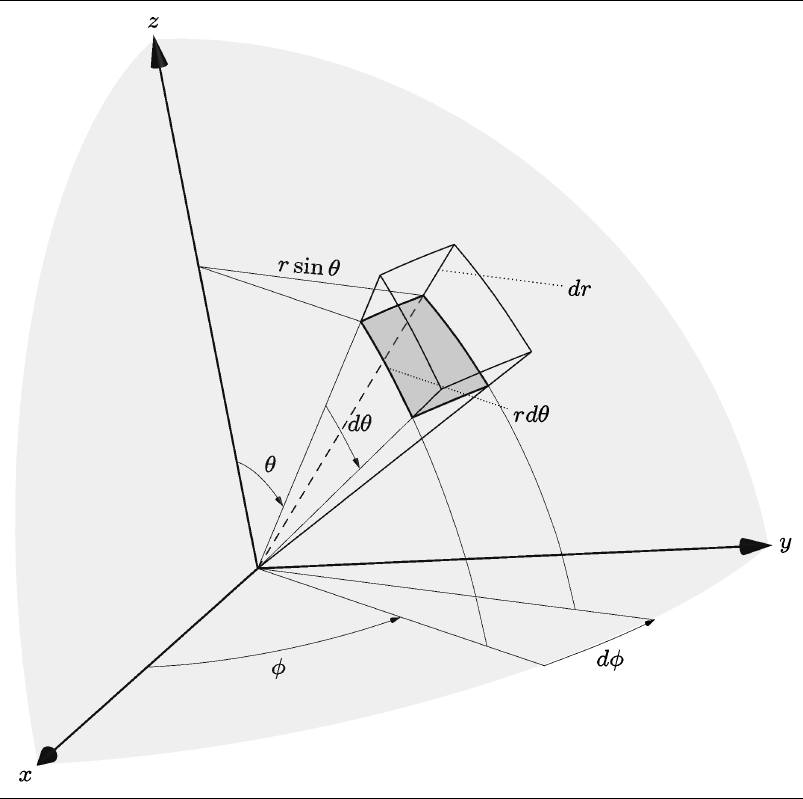
\includegraphics[scale = 0.6]{Chapter2_Theory/images/coordinates.png}
%    \caption{Credit, https://tex.stackexchange.com/questions/159445/draw-in-cylindrical-and-spherical-coordinates}
%    \label{fig:coords}
%\end{figure}
%The cloud cover will be referred to as cloud amount, fraction or simply the clouds.
%%%%%%%%%%%%%%%%%%%%%%%%%%%%%%%%%%%%%%%%%%%%%%%%%%%%%%%%%%%%%
\section{Practical implications - OUTDATED} \label{sec:practical_implications}
It is necessary to have a understanding of the needs of the end product before conducting large machine learning projects. Answering questions like: What will it be used for and how can it be implemented in useful way?

A major downside of the data driven learning approach is the rigid resolution. A trained model can only be used on similar problems, with the same spatiotemporal resolution. For applications like climate models, output comes in a wide range of different resolutions. Before implementing the finished product in a new model of a different resolution, it would need to be retrained on the resolution of the climate model under development. This process involves both remapping of the dataset and retraining the model at the correct resolution. This is a time consuming process involving finding a new set of hyperparameters suitable for the new resolution. % It essentially means starting over.

Once trained on global climate datasets, machine learning models provide fast results even for complex parameterization which is what makes them suitable for the application of climate modelling. Most machine learning packages are developed using Python. \acrfull{esm} are implemented in python. Methods for including the trained parameterizations need to be developed.
 
\subsection{Any implications based on the results presented in this chapter.}
\\ \\
\subsubsection{Licences and Downloading Data} \label{sec:downloading_data}
Scripts for downloading the ERA5 data used in this thesis is available in the project GitHub on \href{https://github.com/hannasv/MS/tree/metos/downloading{\_}RA}{https://github.com/hannasv/MS/tree/metos/downloading{\_}RA}. However you will need to create a CDS-user. Follow the instructions on ECMWF homepages on \textit{how to download ERA5}. There are no scripts available for downloading METEOSAT data this is done using satellite retrievals at EUMETSATs Earth Observation Portal. Its freely available in hourly resolution. Scientist can apply for increased resolution up to 15min. Choose the cloud mask product in grb-format. By running \textbf{X - legg inn filnavn} you can generate your own files for regridding. The supplementary material only include the domain used in this thesis, because of GitHub has a maximum limit allowed for uploading. 
%%%%%%%%%%%%%%%%%%%%%%%%%%%%%%%%%%%%%%%%%%%%%%%%%%%%%%%%%%%%%%%%%%
\\ \\ 
\subsubsection{summary}
This thesis aim to devolop and/or explore methods of parameterising cloud cover based on macro-scale variables like humidity, surface temperature and pressure. Regressing historical observations against macro physical properties which affect clouds. Moving away from the subgrid scale processes. Wish to answar weather there be enough information in humidity, temperature and surface pressure to predict clouds in a time and space.



